\documentclass[acmtog]{acmart}
\usepackage{graphicx}
\usepackage{subfigure}
\usepackage{natbib}
\usepackage{listings}
\usepackage{bm}
\usepackage{amsmath}

\definecolor{blve}{rgb}{0.3372549 , 0.61176471, 0.83921569}
\definecolor{gr33n}{rgb}{0.29019608, 0.7372549, 0.64705882}
\makeatletter
\lst@InstallKeywords k{class}{classstyle}\slshape{classstyle}{}ld
\makeatother
\lstset{language=C++,
	basicstyle=\ttfamily,
	keywordstyle=\color{blve}\ttfamily,
	stringstyle=\color{red}\ttfamily,
	commentstyle=\color{magenta}\ttfamily,
	morecomment=[l][\color{magenta}]{\#},
	classstyle = \bfseries\color{gr33n}, 
	tabsize=2
}
\lstset{basicstyle=\ttfamily}

% Title portion
\title{Assignment 1:\\ {Exploring OpenGL and Phong Lighting}} 

\author{Name:\quad hidden \\ student number:\ hidden
\\email:\quad hidden@shanghaitech.edu.cn}

% Document starts
\begin{document}
\maketitle

\vspace*{2 ex}

\section{Introduction}

In this assignment, the following tasks are finished.

\begin{itemize}
	\item First, the mesh object in the \texttt{assets} folder are loaded into main memory. They are then sent to and processed by the GPU.
	\item Second, keyboard and mouse (cursor moving and scrolling) input are handled to allow us moving around in the scene and watch those objects from any direction we like. 
	\item After that, the phong lighting model is implemented to make the object look more realistic.
	\item Finally, multiple lighting of different kinds are implemented (bonus1), and normal vectors are shown with the help of geometry shader (bonus2).
\end{itemize}


% \begin{itemize}
% \item ... has been down.
% \item ...
% \item ...
% \end{itemize}



\section{Implementation Details}

\subsection{Loading Meshes From File}

First we need to read \texttt{obj} files into our program. We will implement this inside the \texttt{Mesh} class, located in \texttt{src/mesh.cpp} and header file \texttt{include/mesh.h}. The \texttt{Mesh} class contains mainly the following members.

\begin{itemize}
	\item \texttt{std::vector<Vertex> vertices}, which holds the vertices' position.
 	\item \texttt{std::vector<GLuint> indices}, which holds the indices of vertex position and normal of faces.
  	\item \texttt{uint VAO, VBO, EBO}. These are VAO (Vertex Array Object), VBO (Vertex Buffer Object) and EBO (Element Buffer Object) ids, or references number.
\end{itemize}

The constructor reads in a mesh object by calling member function \texttt{void Mesh::loadDataFromFile(const std::string \&path)} to complete that. It reads in a file line by line, checking the first character (which should be \texttt{'\#'}, \texttt{'v'}, \texttt{'n'} or \texttt{'f'}), and then reads in the float or int values and store in vertices and normals.


\subsection{Draw meshes on the screen}

So far, we have read the file to our CPU memory. Then we need to copy these data to GPU memory for further handling. We achieve that with the help of VAO, VBO and EBO. These are implemented in member function \texttt{void init\_objects()}. In detail, the following things are done.

\begin{itemize}
	\item Bound Vertex Attribute. We need to create a VBO object and bind the vector containing vertex attribute to it. We need to create EBO (index buffer object) and do the similar things for the indices. At last we will bind VBO and EBO to VAO.
	\item Write the shader program. In vertex shader, we need to transform the vertices from model space to clip space. In the fragment shader, we need to calculate the color for each pixel. Note that, for simplicity, we will keep the color to be pure white and implement the lighting model in the next step.
	\item Create and compile shader programs. After the shaders are implemented, we need to compile and link them to a shader program. This is implemented in \verb|void initWithCode(...)| member function in \verb|Shader| class. Error handling is also implemented which will output an error message if the compilation fails.
\end{itemize}

\subsection{Handling mouse and keyboard input events}

Now the objects are correctly rendered, but we cannot move them. We listen for input events by defining a callback function and set them using openGL. However, before that, we need to understand perspective projection first.

The input position of vertices stored in VBO is in world space and we need to transform them into clip space. The transformation is done by multiplying the vertex position with 3 matrices: the model matrix, projection matrix and view matrix.

\begin{itemize}
	\item The model matrix can change the object coordinate in the world space. In this project, we won't change the positions, so this matrix will be omitted (or filled with all 1s).
	\item The projection matrix is calculated by \verb|glm::perspective| \verb|(fov, aspect, near, far)| where \verb|fov| is the field of view, \verb|aspect| is the aspect ratio of the screem, \verb|near| is the nearest plane and \verb|far| is the furthest plane.
	\item The view matrix is calculated by \verb|glm::lookAt(camera_pos),| \verb|camera_pos + camera_gaze, camera_up|, where \verb|camera_pos| is the position of the camera, \verb|camera_gaze| is the direction the camera is facing, and \verb|camera_up| is the up direction of the camera.
\end{itemize}

All the three matrices above are calculated in \verb|main.cpp| and then passed into shader programs using uniform variables. The vertex shader multiplies the matrices and transform the vertex position into clip space.

Now back to input handling. There are three callback functions for keyboard, mouse cursor movements and mouse scrollin. To make the code structure easier for management, we implemented a \verb|Camera| class with camera information and camera movement member functions inside it.

There are three callback functions for keyboard, mouse cursor move, and mouse scrolling. 

\begin{itemize}
	\item Keyboard Input.
 
	When any of W,A,S,D,R,F is pressed, we move the camera position. This is done in \texttt{void process\_input(GLFWwindow *win)}. 

	\begin{itemize}
		\item we can move the camera up and down by pressing W or S
		\item we can move the camera left and right by pressing A or D
		\item we can move the camera forward and backward along the gaze direction by pressing R and F
	\end{itemize}

	\item Mouse cursor input.
 
	When mouse is moved, we update \texttt{pitch}, \texttt{yaw}. This is done in \texttt{void my\_mouse\_callback(GLFWwindow *win, double x, double y)}. Note that since we need to get the mouse movement instead of mouse position at each time, we have to set a \texttt{bool firstMouse} flag, which is initialized to be true. In the first mouse callback, we store the current mouse position. Otherwise, we check for mouse movement scale and update the current position.

	Then we bind this function by \texttt{glfwSetCursorPosCallback} before entering the main loop.


	\item Mouse scrolling movement.
 
	We will update \texttt{fov} (field of view) when mouse scrolling is detected. We bind this by \texttt{glfwSetScrollCallback} before entering the main loop.

	\item Disable cursor.
 
	Finally we disable the cursor display (so that we will not see the cursor while moving our mouse) by \texttt{glfwSetInputMode}.
 

\end{itemize}


\subsection{Phong shading model implementation}

So far, we have successfully drawn the object shape, but it is in pure orange color. We need to add lighting to it. Fragment shader controls the behavior of each fragment, so we will mainly implement the phong lighting in \texttt{fShader.glsl} file.

According to phong lighting model, the color of a fragment is the sum of ambient light, diffuse light and specular light.

\begin{itemize}
	\item Ambient light. This comes from the reflection of the environment. It is independent of the surface normal. We will use a constant factor of \verb|0.2|.
	\item Diffuse light. The diffuse light depends on the relations between the light source and the object. We calculate the dot product of light direction and normal vector (of a fragment) to get the strength of diffuse color.
	\item Specular light. We use the \verb|reflect| function to calculate the reflection of light direction and normal vector, and then adding the view matrix.
\end{itemize}


\subsection{Geometry shader}

The geometry shader is an optional shader stage that sits between the vertex and fragment shaders. It can convert the original primitives to completely different primitices. In this assignment, we will show the normal vectors of the object using this shader. 

We will implemented another combination of shaders (with geometry shader) and compile these two shaders. Then inside the main loop, we will use the original shader first, and then apply this geometry shader.



\section{Results}

\subsection{Basic Phong lighting model and multiple light sources}

Here are the front and back side of the bunny. There's a bright and yellow light source in the front, and a darker pink light source in the back.

\begin{figure}[H]
	\centering
	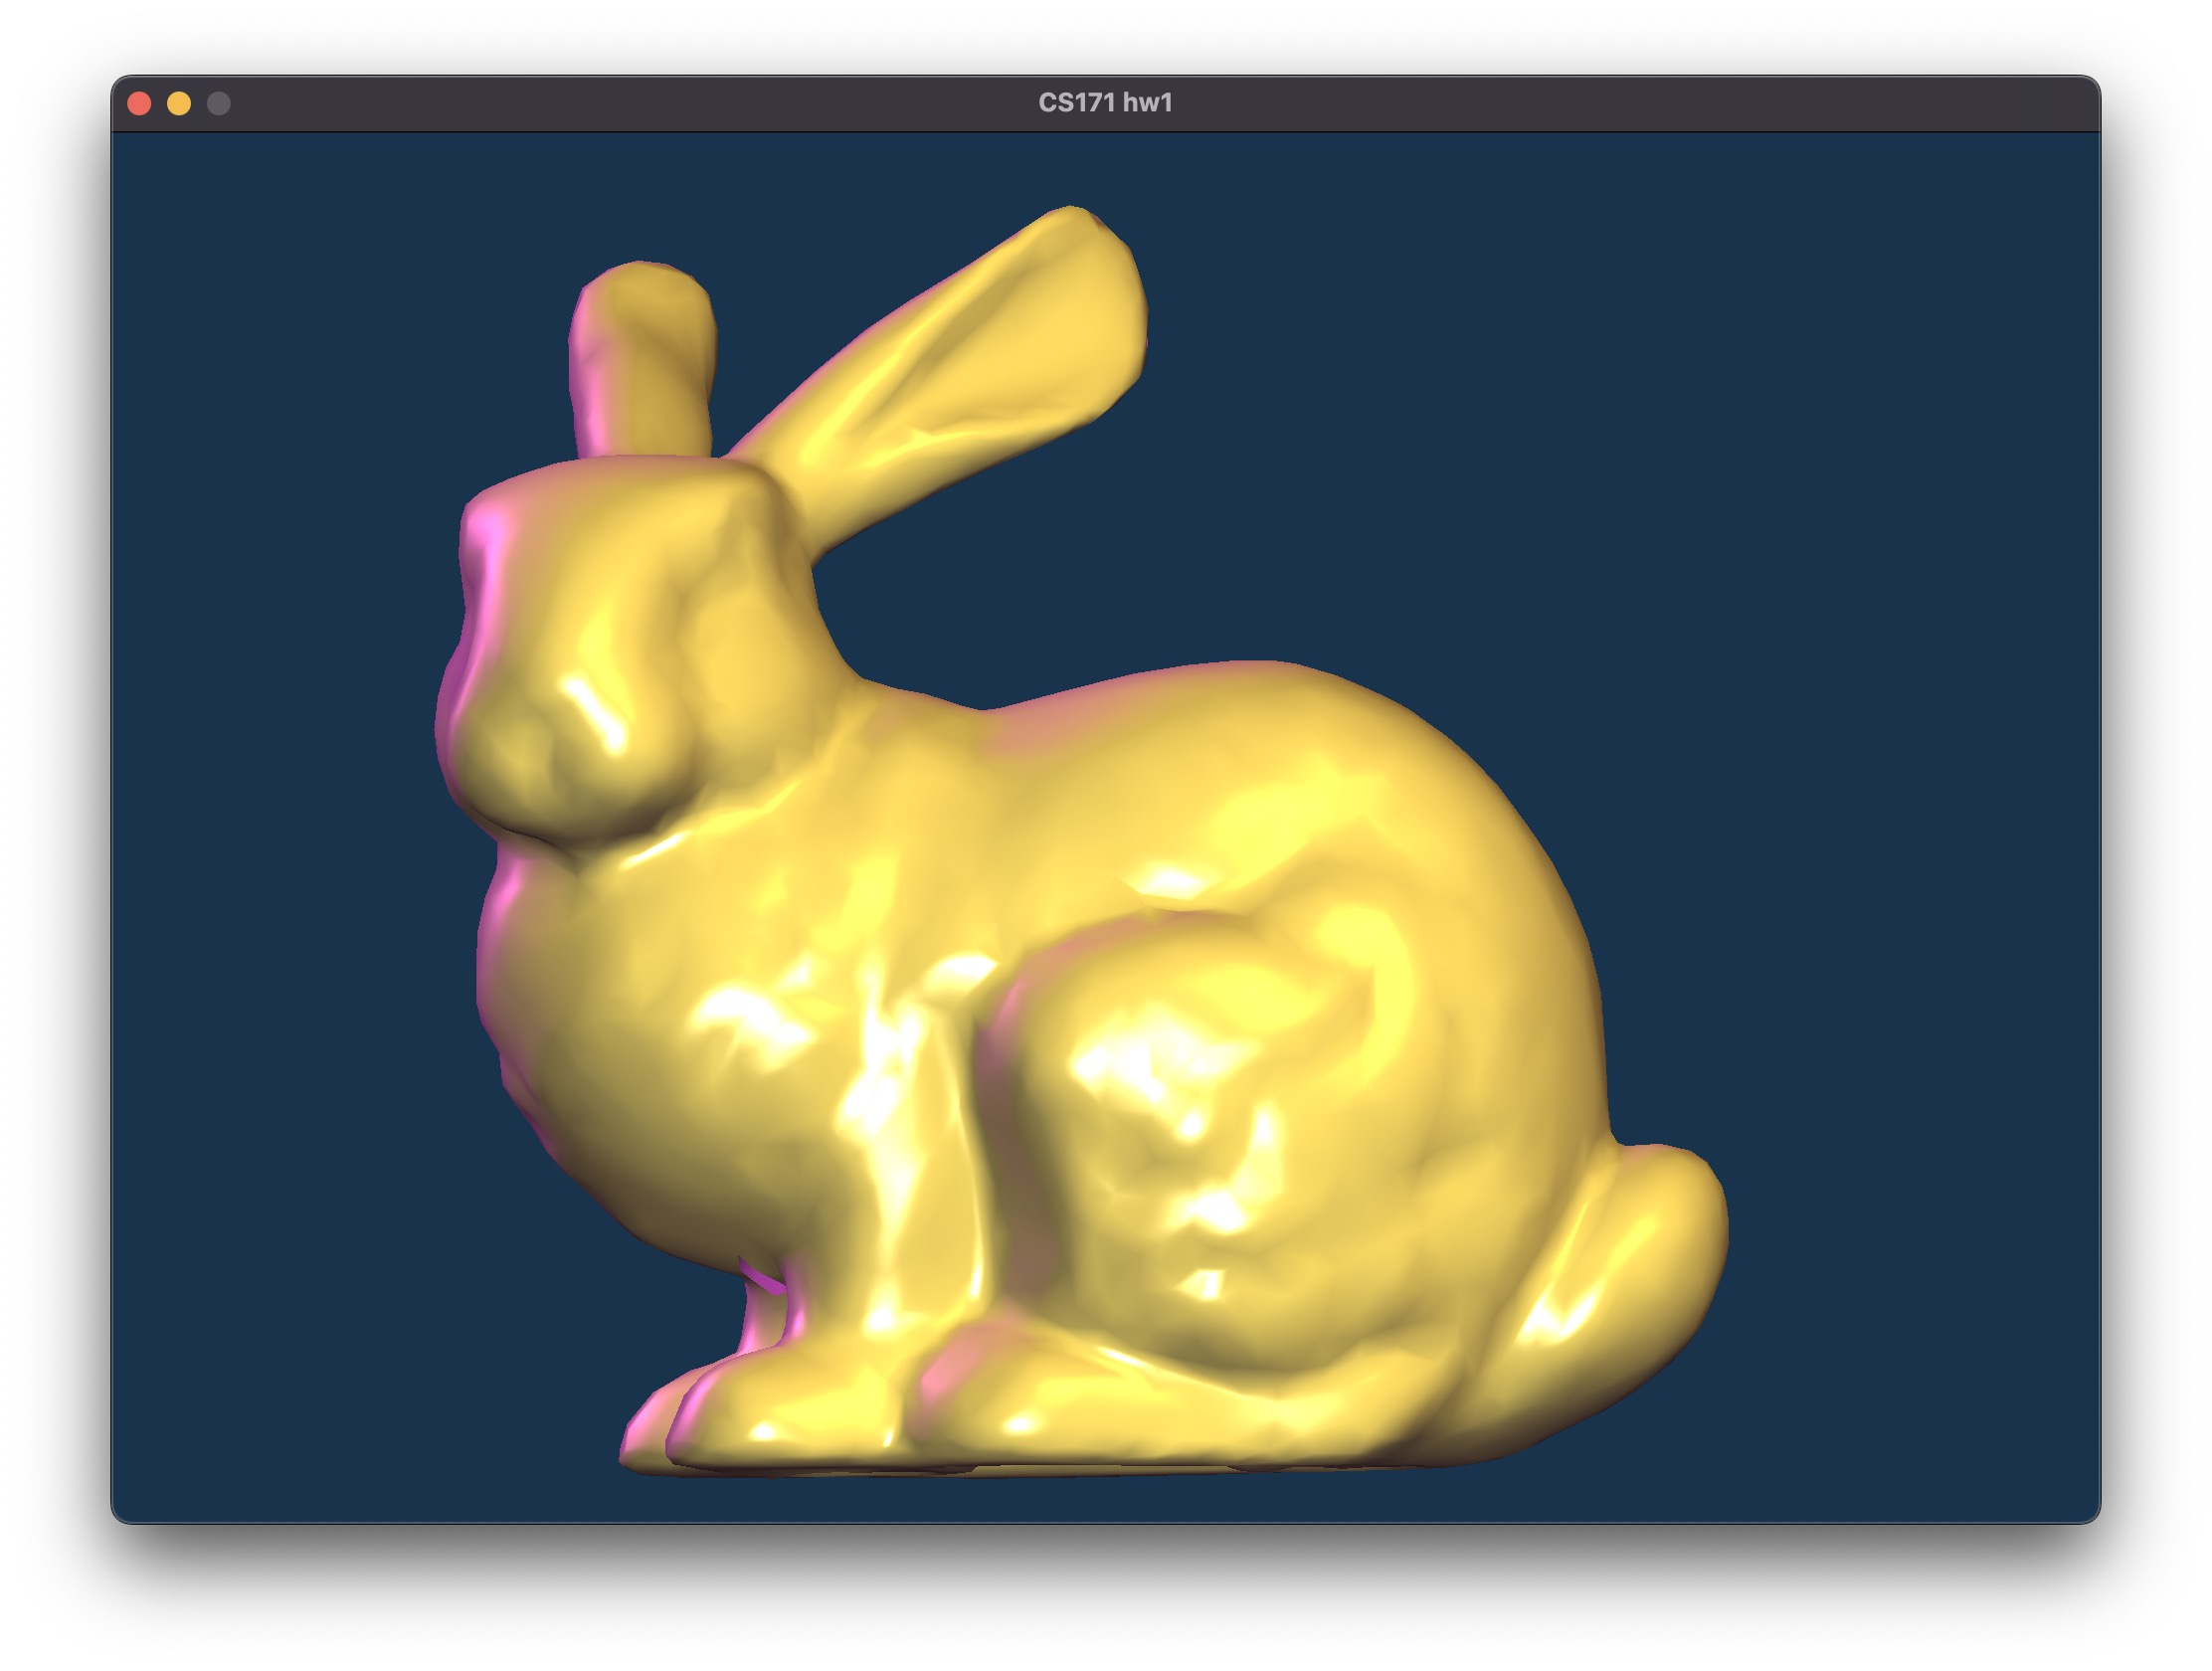
\includegraphics[scale=0.08]{pictures/front.jpg}
	\caption{Front side of the bunny}
% \end{figure}

% \begin{figure}[H]
	\centering
	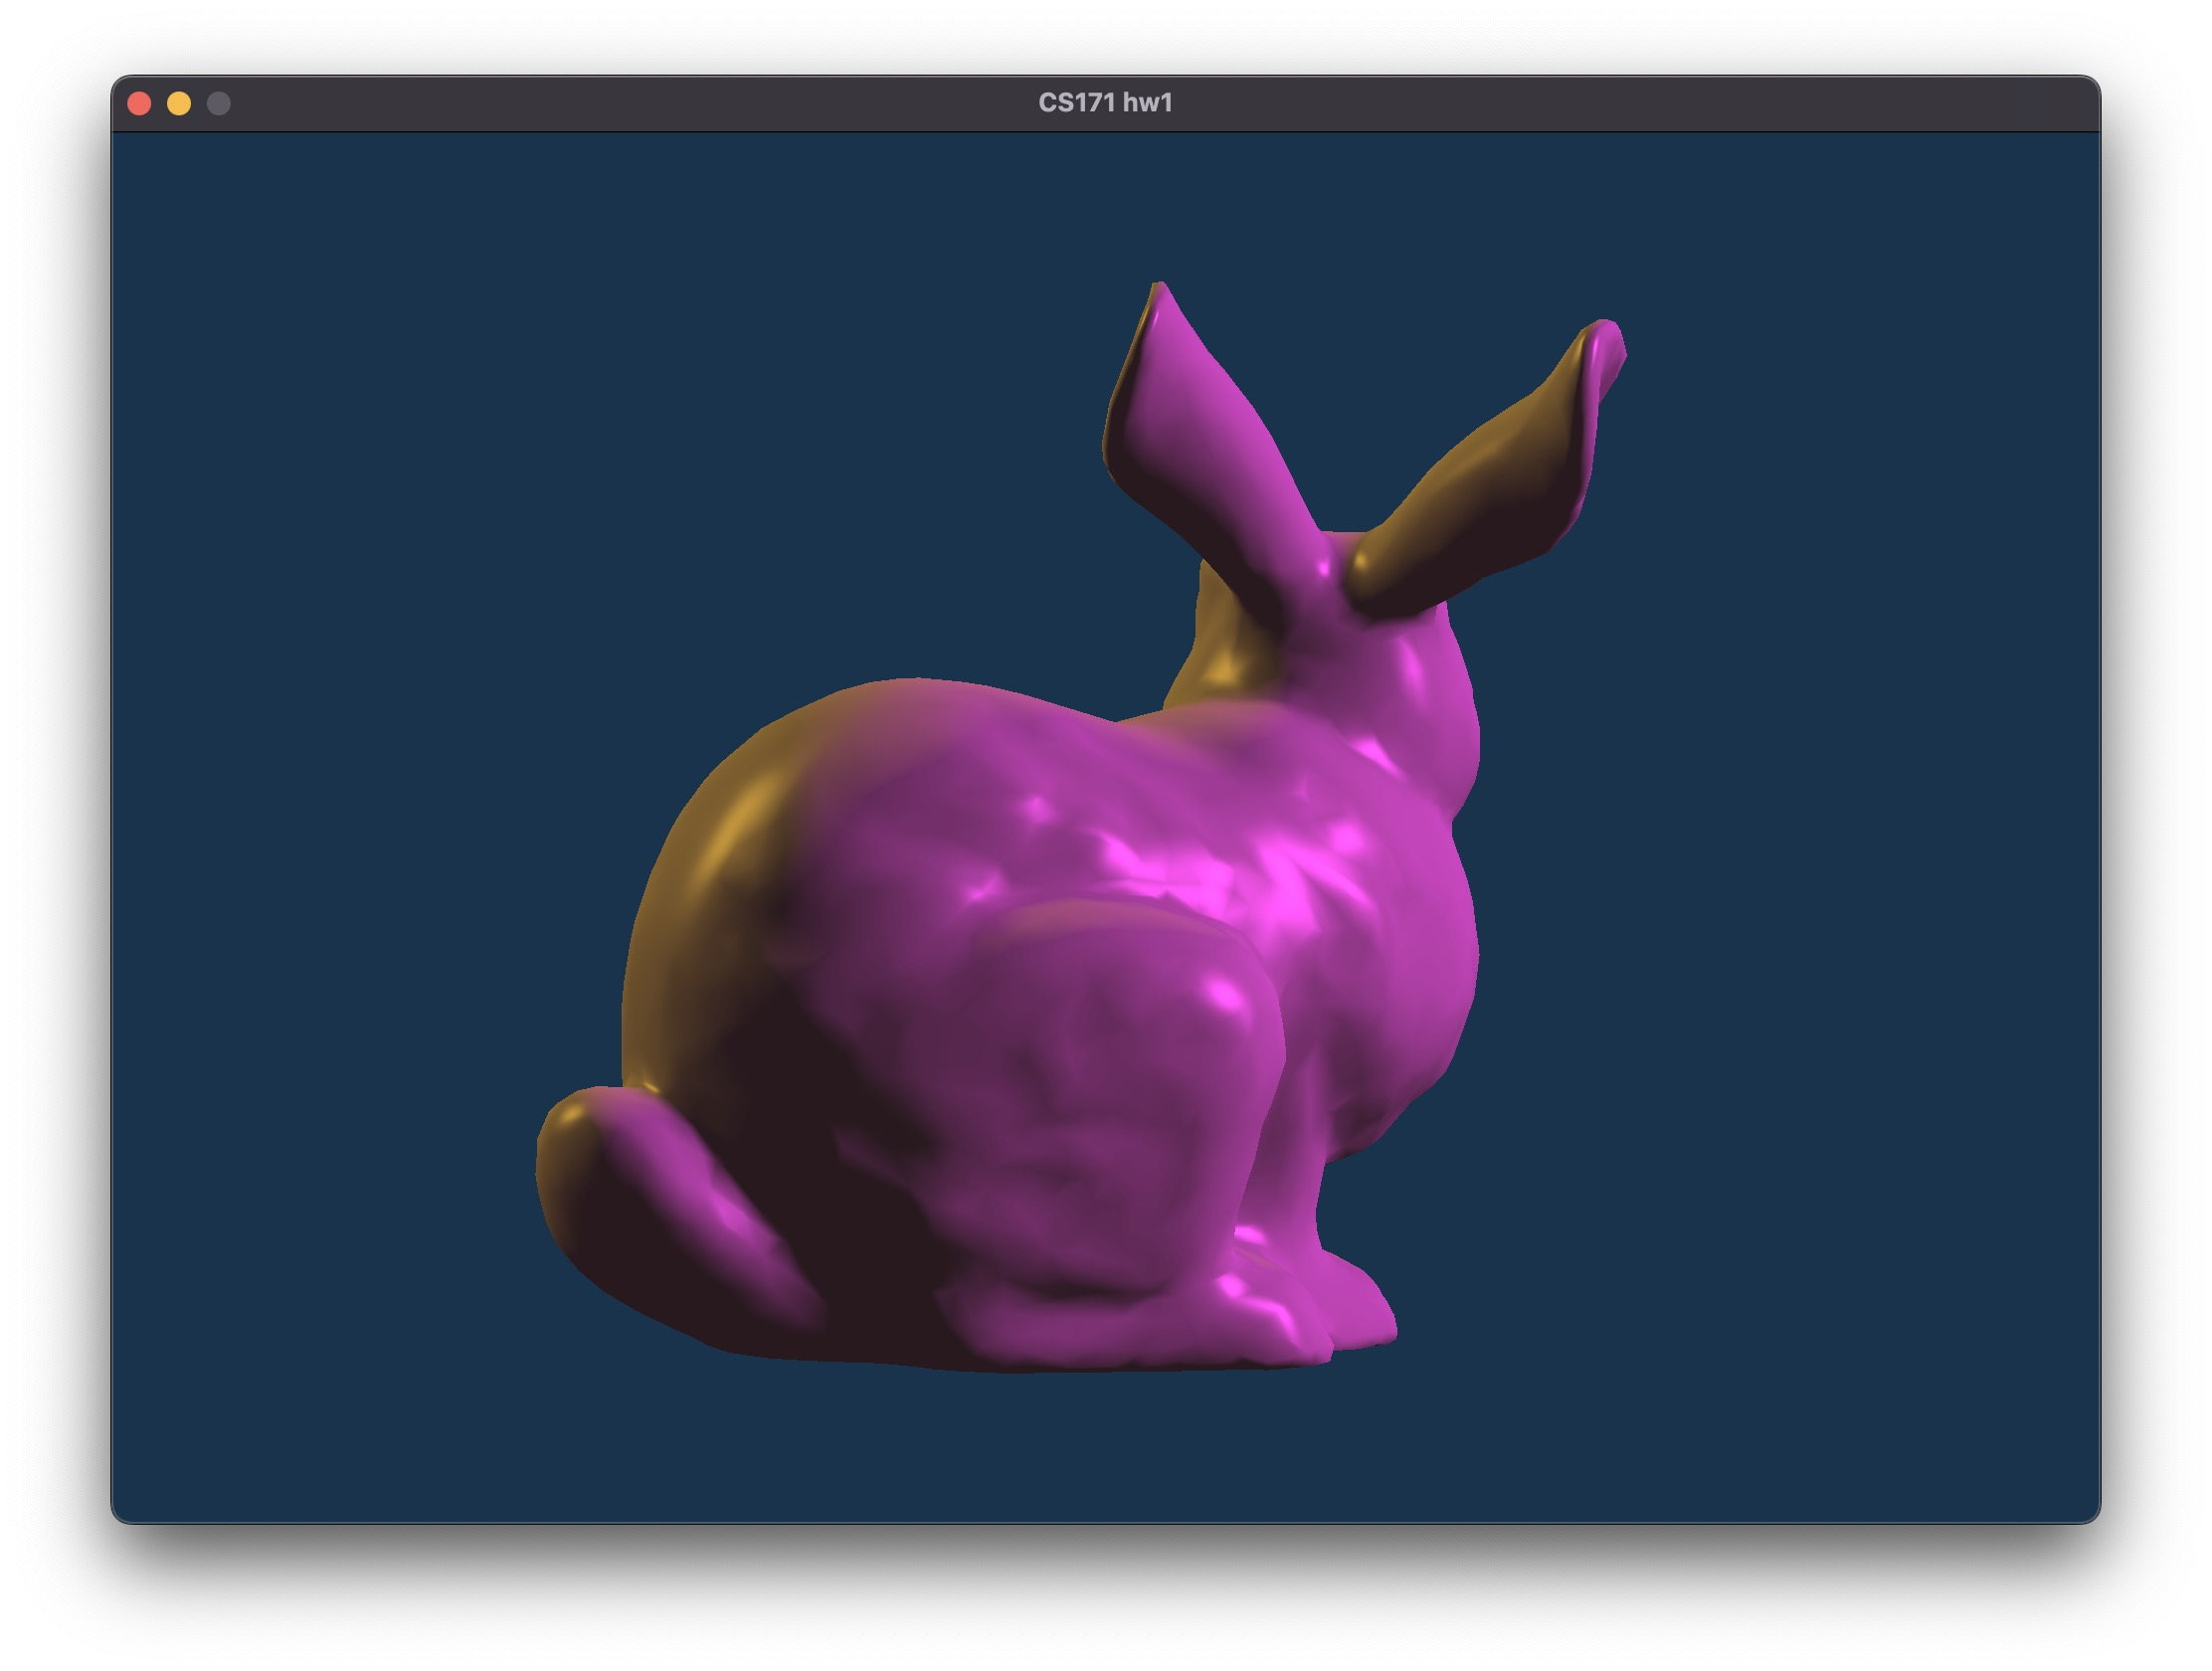
\includegraphics[scale=0.08]{pictures/back.jpg}
	\caption{Back side of the bunny}
\end{figure}


\pagebreak
\subsection{Spotlight}

There's also a spotlight shining from the camera. When we move the bunny slowly away from the spotlight, we can see its surface darkening.

\begin{figure}[h]
	\centering
	\subfigure[under spotlight]
	{
		\begin{minipage}[b]{.4\linewidth}
			\centering
			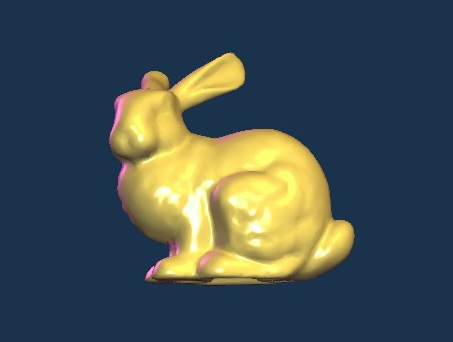
\includegraphics[scale=0.6]{pictures/under_spotlight.jpg}
		\end{minipage}
	}\\
	\subfigure[halfway outside spotlight]
	{
		\begin{minipage}[b]{.4\linewidth}
			\centering
			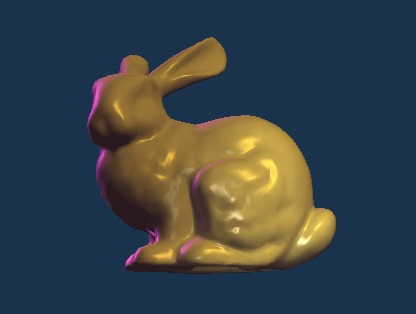
\includegraphics[scale=0.66]{pictures/half_outside_spotlight.jpg}
		\end{minipage}
	}\\
	\subfigure[outside spotlight]
	{
		\begin{minipage}[b]{.4\linewidth}
			\centering
			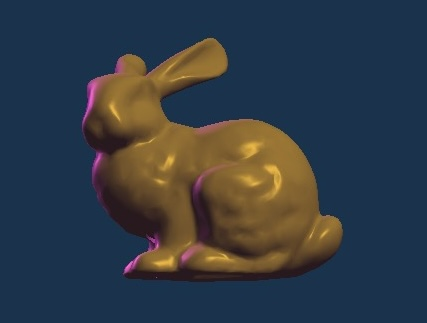
\includegraphics[scale=0.66]{pictures/outside_spotlight.jpg}
		\end{minipage}
	}
	% \\
	\caption{Spotlight}
\end{figure}


\pagebreak

\subsection{Geometry shader and Normal vector}

By implementing a geometry shader, we can show the bunny's normal vectors.

\begin{figure}[H]
	\centering
	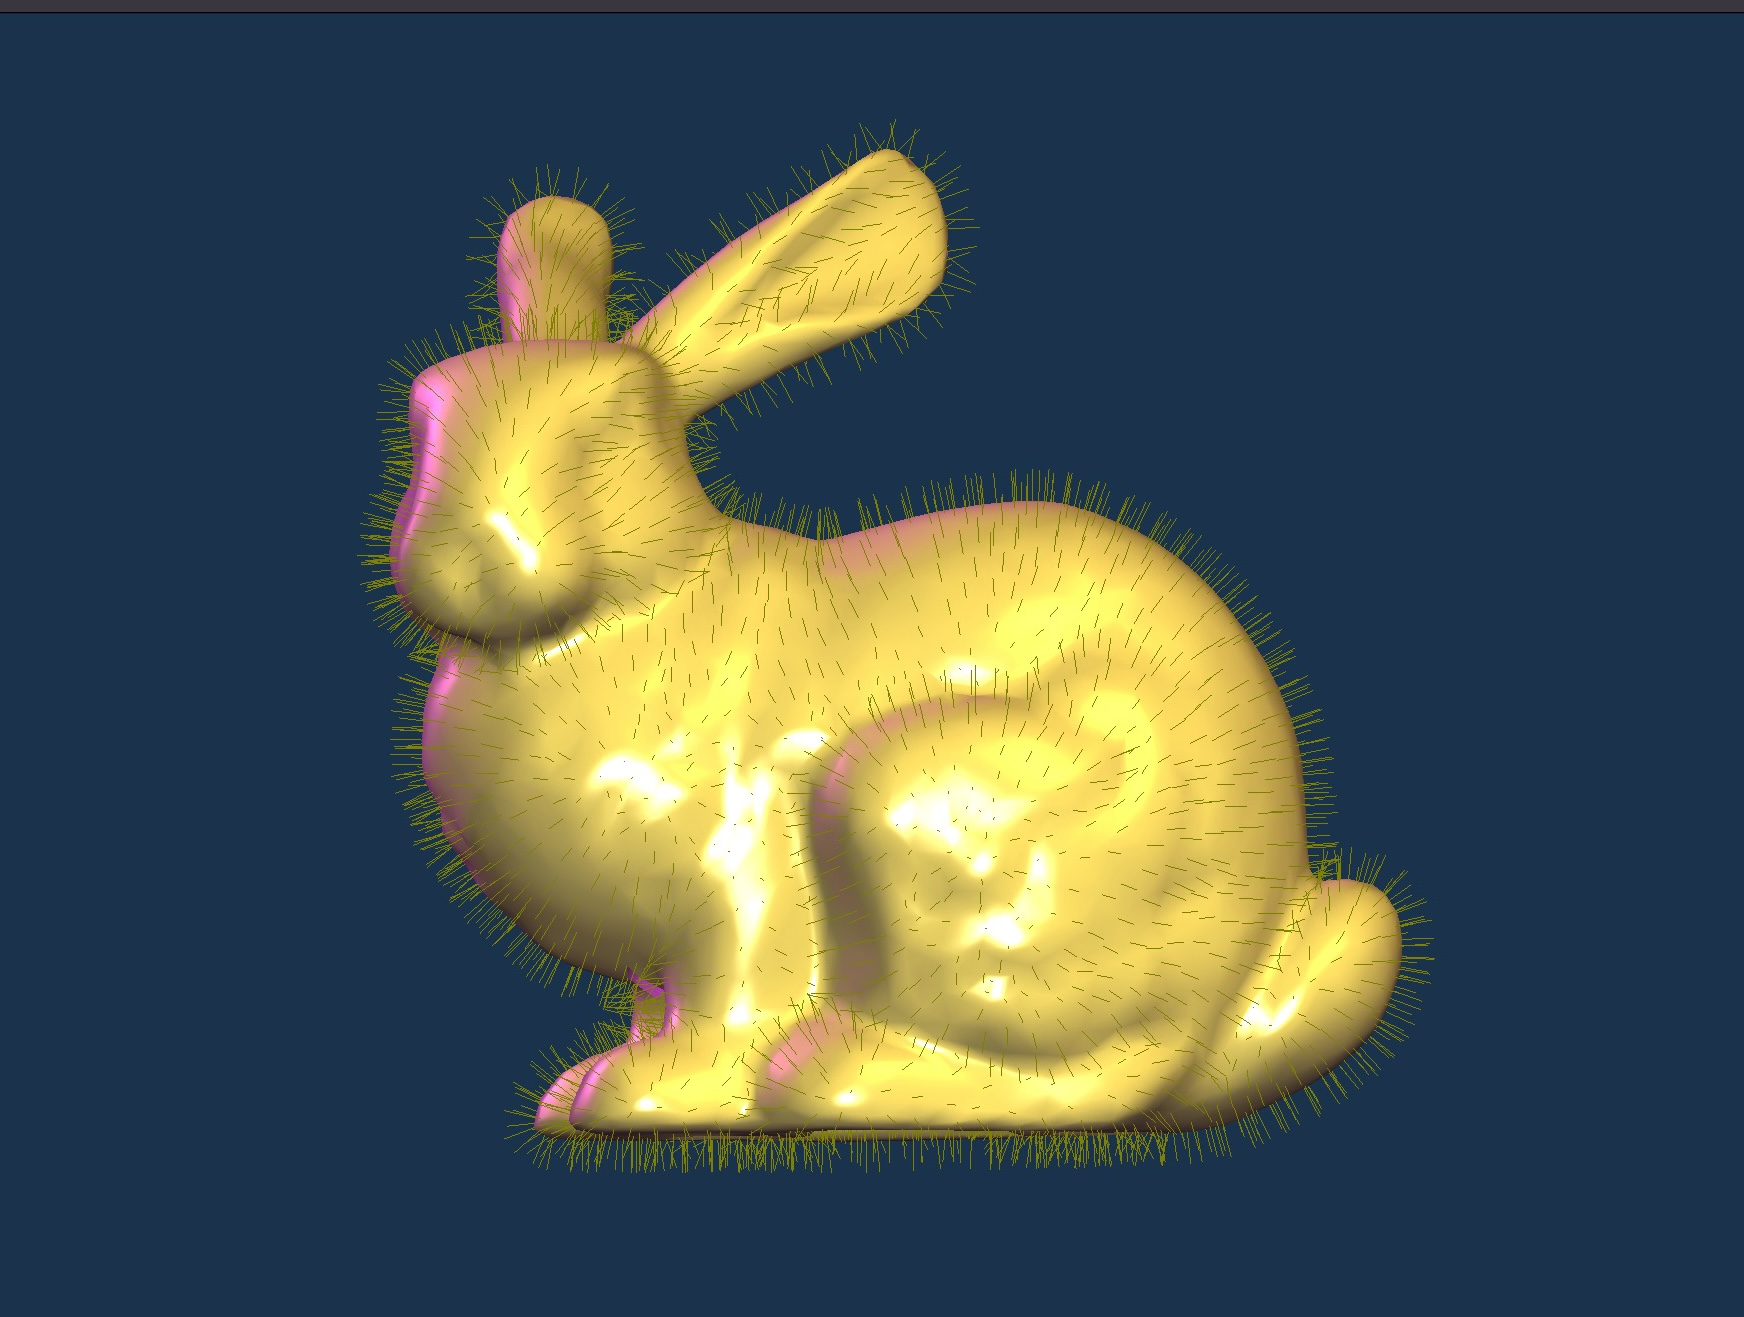
\includegraphics[scale=0.2]{pictures/fur.jpg}
	\caption{Bunny with its normal vectors as fur}
\end{figure}

\begin{figure}[H]
	\centering
	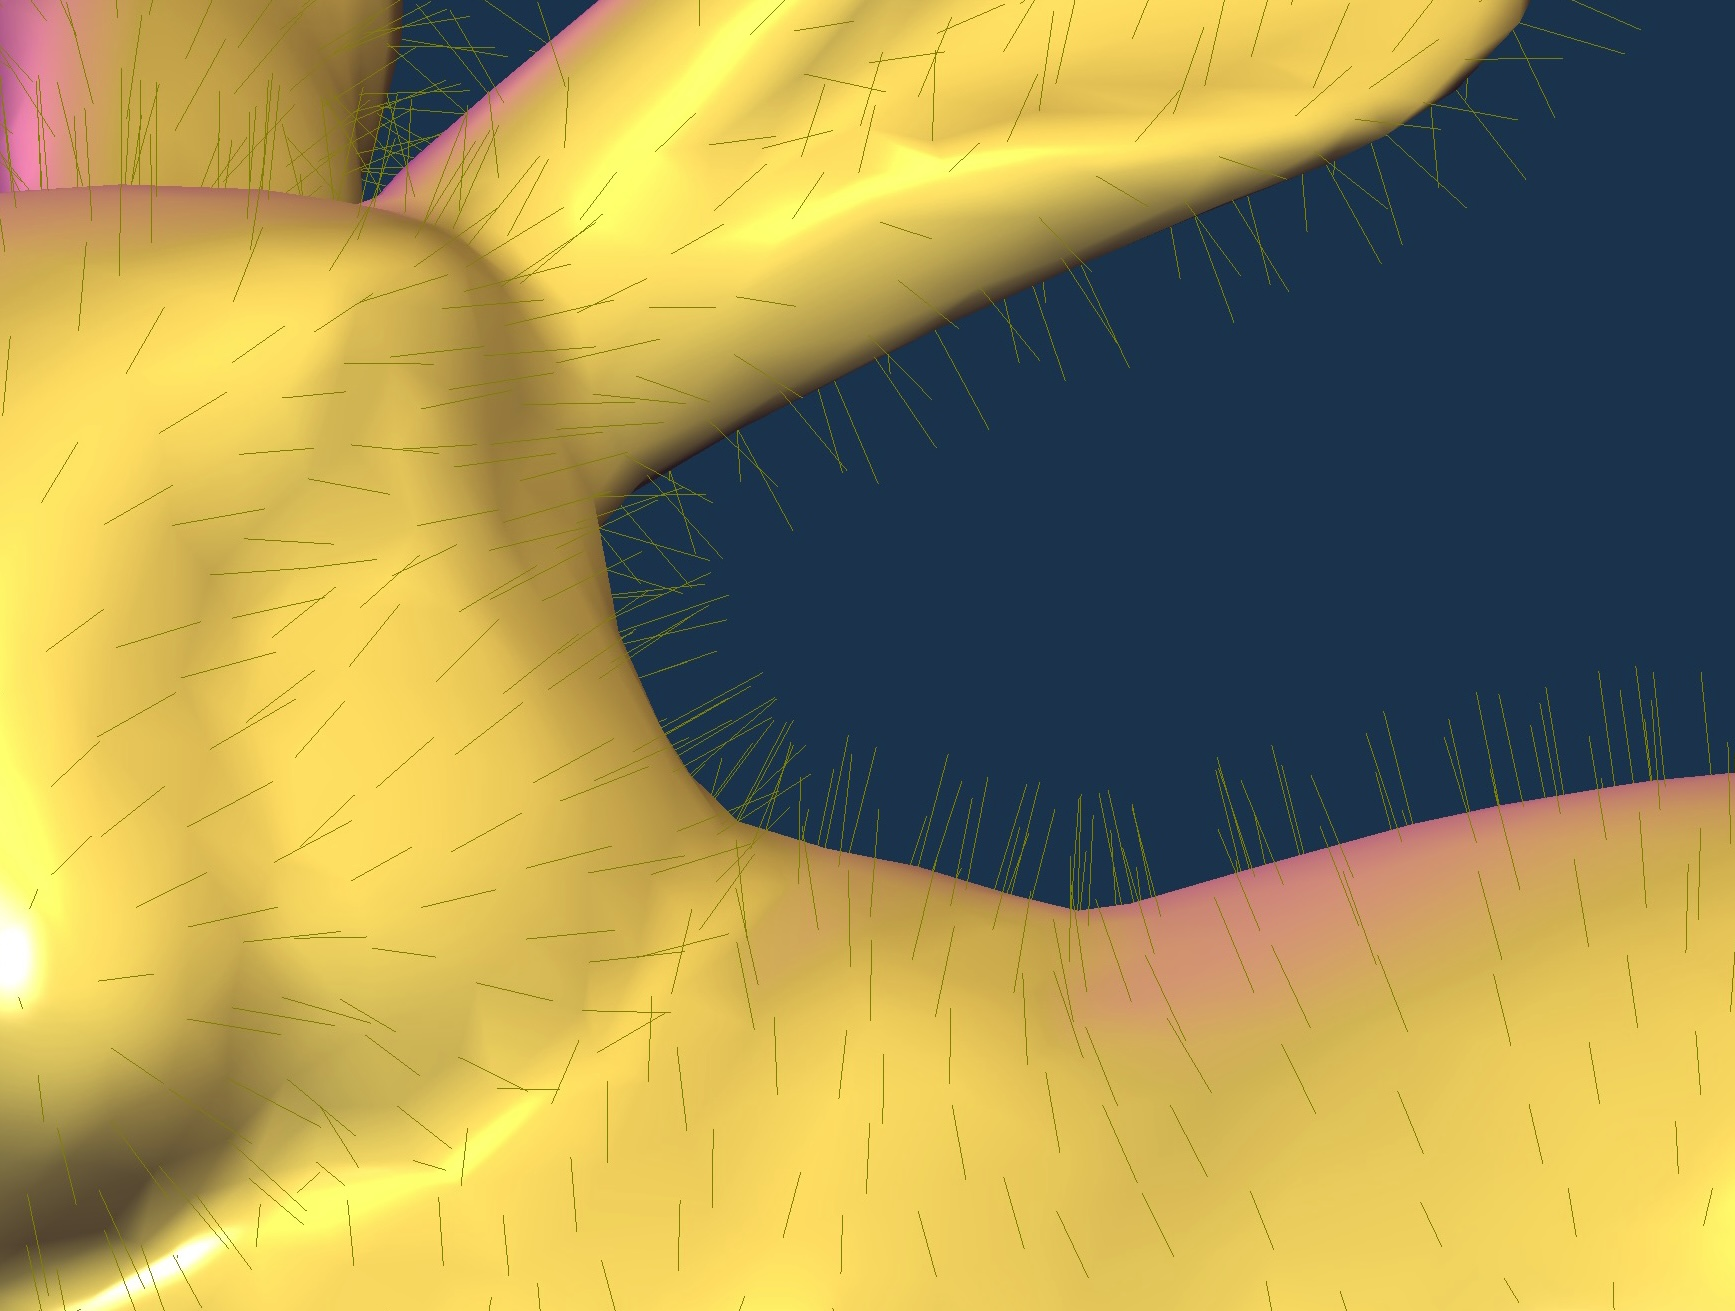
\includegraphics[scale=0.2]{pictures/fur-details.jpg}
	\caption{Details of the above}
\end{figure}


\end{document}
